% This is LLNCSDOC.TEX, the documentation file of
% the LaTeX2e class from Springer-Verlag
% for Lecture Notes in Computer Science, version 2.24
\documentclass[runningheads]{llncs}
% Add PDF bookmarks and metadata
\usepackage[bookmarksopen,
bookmarksopenlevel=1,
bookmarksdepth=2,
pdftex,
pdfauthor={No Author Given},
pdftitle={Instantaneous, Comprehensible, and Fixable Soundness Checking of Industrial BPMN Models},
pdfsubject={BPMN soundness checking},
pdfkeywords={BPM, Verification, Soundness, Safeness}
]{hyperref}
%
\usepackage{graphicx}
% Modern tables
\usepackage{tabularray}

\begin{document}
%
\title{Instantaneous, Comprehensible, and Fixable Soundness Checking of Realistic BPMN Models}
%
\titlerunning{Instantaneous, Comprehensible, and Fixable BPMN Soundness Checking}
% \author{Tim Kr\"{a}uter\inst{1}\orcidID{0000-0003-1795-0611} \and
% Adrian Rutle\inst{1}\orcidID{0000-0002-4158-1644} \and
% Harald K\"{o}nig\inst{2,1}\orcidID{0000-0001-6304-6311} \and
% Yngve Lamo\inst{1}\orcidID{0000-0001-9196-1779}}
% TODO: Patrick
% \authorrunning{T. Kräuter et al.}
% \institute{Western Norway University of Applied Sciences, Bergen, Norway
% \email{tkra@hvl.no, aru@hvl.no, yla@hvl.no} \and
% University of Applied Sciences, FHDW, Hanover, Germany\\
% \email{harald.koenig@fhdw.de}}
%
\maketitle              % typeset the header of the contribution
%
\begin{abstract}
	
Many business process models have control-flow errors, such as deadlocks, which can hinder code generation and proper execution.
In this paper, we introduce our new soundness checking tool that can instantaneously identify errors in BPMN models, make them comprehensible for modelers, and even suggest fixes to eliminate them automatically.
We demonstrate that our tool's soundness checking is instantaneous, taking less than 500ms, by benchmarking our tool against synthetic BPMN models with increasing size and state space complexity, as well as realistic models provided in the literature.
Moreover, the tool directly displays possible soundness violations in the modeler and provides an interactive token-flow animation illustrating each violation.
Additionally, it provides fixes to resolve the violations found, which, to the best of our knowledge, is not currently available in other tools.
The tool is open-source, modular, extensible, and smoothly integrated into a BPMN editor.

\keywords{
BPM \and
Verification \and
Soundness \and
Safeness
}
\end{abstract}

% Up to 16 pages, including everything!

% Redefine enumerations
\renewcommand{\labelenumi}{(\textbf{\arabic{enumi})}}

\section{Introduction} \label{sec:introduction}

% Problem statement
% Why useful? Check
\cite{fahlandAnalysisDemandInstantaneous2011}
% Claims a lot of problems in workflow models, which can be found using soundness checks.

% Motivation

% Solution
% Describe the figure and go over all three claims briefly: instantaneous (Definition), comprehensible (soundness properties are hard to understand for modelers), and  (comparable to quick fixes).

% Also add the times measured by other tools for some models. These range into seconds. It would be nice to try the same models later.

% Comprehensible/Visualization is missing in the figure: instantaneous and fixable are there.
\begin{figure}[ht]
	\centering
	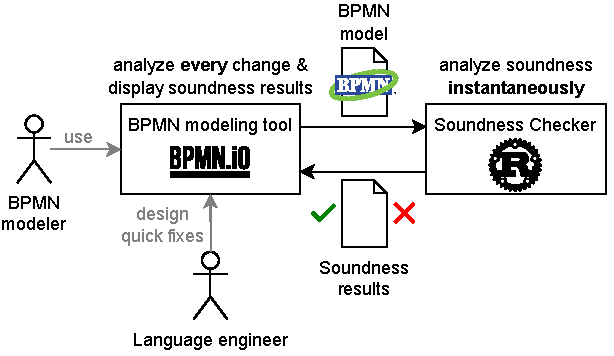
\includegraphics[width=0.7\textwidth]{images/overview}
	\caption{Overview of the approach}
	\label{fig:overview}
\end{figure}

% What do the results contain? If wrong: Counterexample and problematic elements

% Soundness stuff taken from which adopted it for BPMN
\cite{corradiniClassificationBPMNCollaborations2018}

% One example should be introduced here, which then is picked up throughout the paper.
% Wrong gateway usage?
% Instantaneous: The model checks in 500ms or less.
% Comprehensible: Highlight problematic elements + show the visualization of a counterexample using that model.
% Fixable: Provide quick fixes that resolve soundness violation --> check if changes fix the property before showing it to the user.

\section{Soundness Checking of BPMN Models} \label{sec:soundness}

% Describe soundness checking for BPMN models.
Soundness was introduced for workflow nets in \cite{vanderaalstAPPLICATIONPETRINETS1998} and stems from the field of Petri Nets.
We will use the formal definition directly given for BPMN by \cite{corradiniClassificationBPMNCollaborations2018}.

% Soundness does not include safeness.
Soundness is composed of three following sub-properties \cite{corradiniClassificationBPMNCollaborations2018}:
\textit{(i) Option to complete}: any running process instance must eventually complete,
\textit{(ii) Proper Completion}: at the moment of completion, each token of the process instance must be in a different end event and
\textit{(iii) No dead activities}: any activity can be executed in at least one process instance.
In addition, we also check \textit{safeness}.
A BPMN model is \textit{safe} if, during its execution, no more than one token occurs along the same sequence flow \cite{corradiniClassificationBPMNCollaborations2018}.

In the remainder of this section, we describe how we achieve \textit{instantaneous}, \textit{comprehensible}, and \textit{fixable} soundness checking of realistic BPMN models.


\subsection{Instantaneous Soundness Checking} \label{subsec:instantaneous}
\textit{Instantaneous} soundness checking is defined as taking 500 ms or less in~\cite{fahlandAnalysisDemandInstantaneous2011}.
In this section, we demonstrate that our soundness checker is instantaneous by validating it from three viewpoints.
First, we investigate how our tools react to rapidly \textit{growing model size}.
We use a benchmark based on synthetically generated BPMN models.
Second, we study how our tool deals with a \textit{growing number of parallel branches} of varying size.
Third, we run soundness checking for realistic BPMN process models available in the literature and public datasets.

% General info
% We use hyperfine for each benchmark with runs stuff 10x and averages. See my other papers
For all our benchmarks, we use the hyperfine benchmarking tool~\cite{peterHyperfine2023} (version 1.18.0), which calculates the average runtime when executing each soundness check ten or more times.
The benchmarks were run on the Windows Subsystem for Linux (WSL) with an AMD Ryzen 7700X processor and 32 GB of RAM.
% Artifacts using a Zenodo link at the end. Anonymous GitHub account before.
All used BPMN models and our tools to generate them are given in the artifacts of this paper~\cite{noauthorgivenBPM2024Artifacts2024}.
Furthermore, we provide the scripts to replicate our benchmarks.

\subsubsection{Growing Model Size}
We use the data set of models provided in~\cite{krauterHigherorderTransformationApproach2023}, which consists of 300 synthetically generated BPMN models, and extend it to 500 models.
% Briefly recap the method.
Every BPMN model contains a start event, a fixed amount of \textit{blocks}, and an end event.
The number of blocks ranges from 1 to 500, and three unique blocks are used repeatedly.
For example, \autoref{fig:three-block-example} shows the third BPMN model in the data set, which contains each block once ~\cite{krauterHigherorderTransformationApproach2023}.
We then progressively add more blocks to the models until we reach 500.
We provide a tool to generate models such as \autoref{fig:three-block-example} and the 500 models itself~\cite{noauthorgivenBPM2024Artifacts2024}.

\begin{figure}[ht]
	\centering
	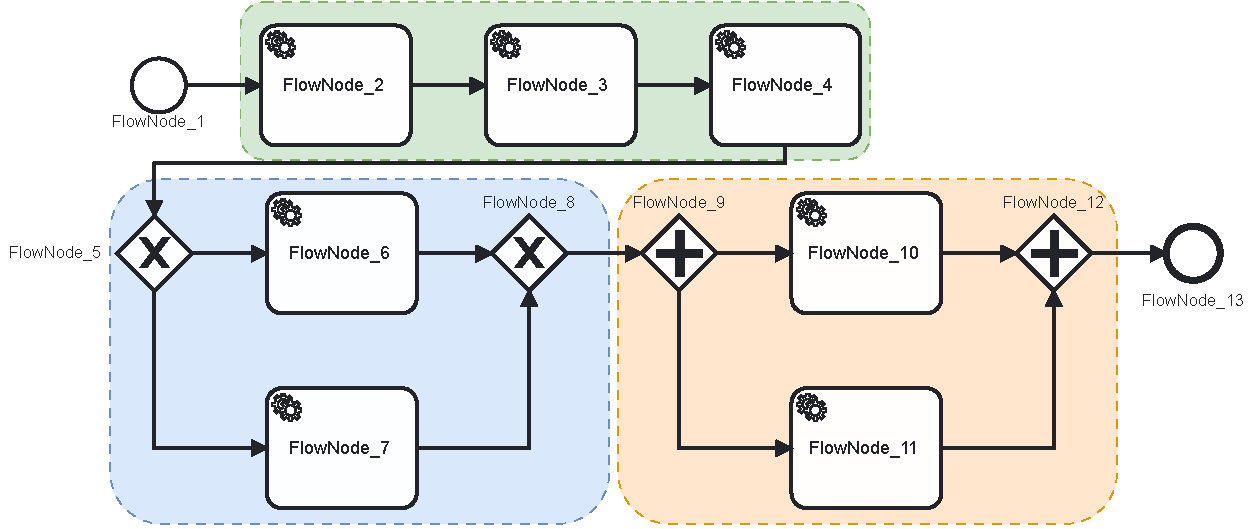
\includegraphics[width=0.8\textwidth]{images/three-blocks}
	\caption{BPMN model with three blocks~\cite{krauterHigherorderTransformationApproach2023}}
	\label{fig:three-block-example}
\end{figure}

\autoref{fig:model-size-benchmark} shows the average runtime of our tool when checking soundness and safeness for the BPMN models with increasing model size.
Our tool explores the entire state space while simultaneously verifying all properties.

\begin{figure}[ht]
	\centering
	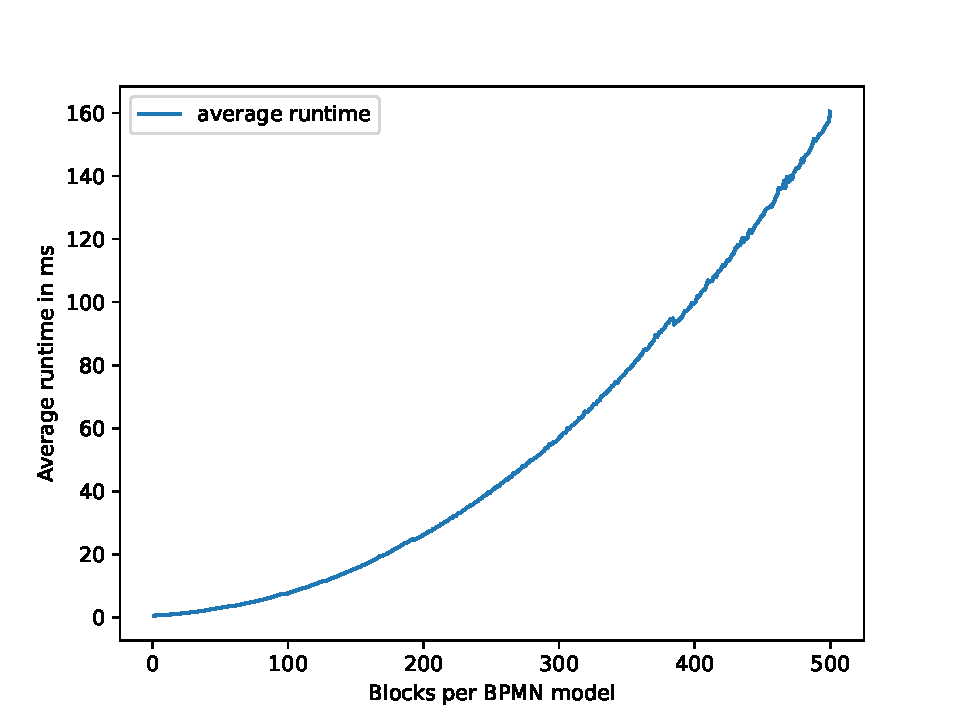
\includegraphics[width=0.6\textwidth]{images/model-size-benchmark}
	\caption{Soundness checking runtime for models of increasing size}
	\label{fig:model-size-benchmark}
\end{figure}

% Results
One can see that our tool spends from 20 ms up to 128 ms for the BPMN models.
Thus, our tool can check soundness \textit{instantaneously} (runtime below 500 ms) even if the model size increases to over 4000 BPMN elements (500 blocks).
Models of this size are not human-readable anymore and are usually divided into smaller models according to best practices \cite{fahlandAnalysisDemandInstantaneous2011}.
Thus, models found in practice are likely to be smaller than in our benchmark.
However, they might be more complex, leading to a larger state space, as discussed in the next section.
% States for the previous:
% 1: 5, 5
% 50: 218, 218
% 100: 434, 434
% 150: 652, 652
% 200: 868, 868
% 250: 1084, 1084
% 300: 1302, 1302
% 500: 2168, 2168

\subsubsection{Growing Number of Parallel Branches}
% Cite the other paper here with parallelism and introduce the set of models.
An increased model size leads to a bigger state space that must be analyzed.
In the previous section, a linear increase in model size led to a similar growth in the state space.
However, models with a growing number of parallel branches lead to an exponential increase in the state space, i.e., a state space explosion~\cite{valmariStateExplosionProblem1998}.
In this section, we benchmark our tool against a synthetic data set of models that lead to a state space explosion.
This represents a \textit{worst case} scenario for soundness checking tools.

We generated a data set of models~\cite{noauthorgivenBPM2024Artifacts2024} with a growing number of parallel branches of increasing length, similar to~\cite{corradiniFormalApproachAnalysis2021}.
\autoref{fig:parallel-branches-models} depicts how a model with \textit{n} parallel branches with length \textit{m} is generated.
We provide a tool to generate models as shown in \autoref{fig:parallel-branches-models} and the models itself~\cite{noauthorgivenBPM2024Artifacts2024}.

\begin{figure}[ht]
	\centering
	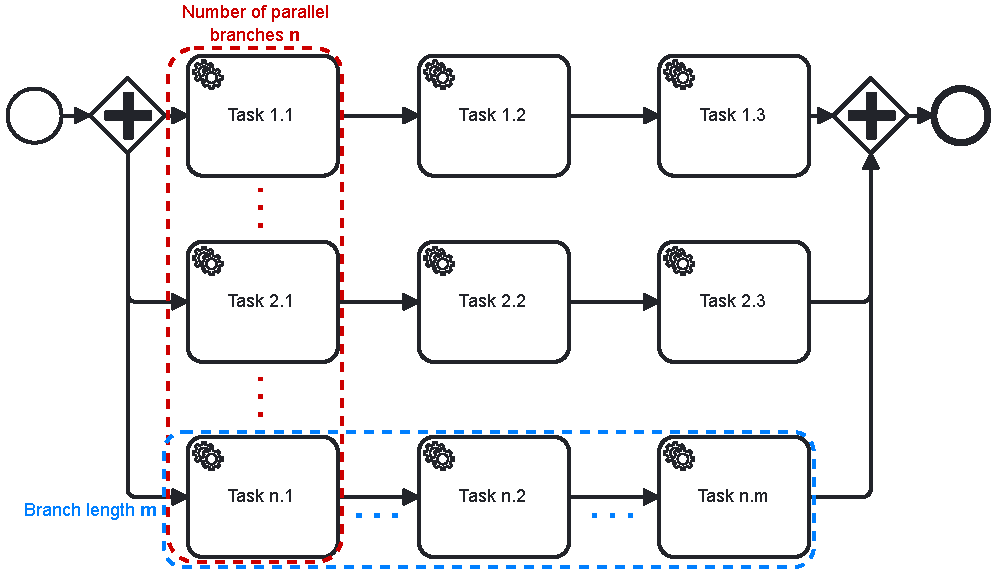
\includegraphics[width=0.8\textwidth]{images/parallel-branches}
	\caption{Models with a growing number of parallel branches and branch length}
	\label{fig:parallel-branches-models}
\end{figure}

\autoref{tab:parallel-branches-benchmark} shows the average runtime of our tool when checking soundness and safeness for BPMN models with a varying number of parallel branches and branch lengths.
Our tool explores the entire state space while simultaneously verifying all properties.

\begin{table}
	\centering
	\caption{Benchmark results of the parallel branches models}
	\label{tab:parallel-branches-benchmark}
	\SetTblrInner{colsep=2pt}
	\begin{tblr}{
			column{1-X} = {c},
			column{Y-Z} = {r},
			hline{1, 2, Z} = {-}{1.2pt, solid}, % Z is the last row/column
			hline{8, 10} = {-}{dashed},
			vline{2-Y} = {2-Z}{solid}, % Y is the second to last row/column
		}
		\textbf{Branches} & \textbf{Branch Length} &\textbf{Runtime} & \textbf{States} \\
		5 & 1 & 20 ms& 35 \\
		10 & 1 & 25 ms& 1.027 \\
		15 & 1 & 388 ms& 32.771 \\
		16 & 1 & 860 ms& 65.539 \\
		17 & 1 & 1.886 ms& 131.075 \\
		20 & 1 & 20.719 ms& 1.048.579 \\
		5 & 3 & 23 ms& 1.027 \\
		5 & 5 & 48 ms& 7.779 \\
		3 & 10 & 23 ms& 1.334 \\
		3 & 20 & 50 ms& 9.264 \\
	\end{tblr}
\end{table}

The state space of the models grows exponentially (in our case, the number of states is given by $(m+1)^n + 3$), clearly showing state space explosion.
Thus, our analysis is not instantaneous anymore when approaching 16 parallel branches of length 1 (see \autoref{tab:parallel-branches-benchmark}).
However, analysis is still instantaneous for more reasonable models with five parallel branches of length 5 or 3 parallel branches of length 10-20.
We believe that models with a high degree of parallelism, such that analysis is not instantaneous, are the exception, not the rule.

\subsubsection{Realistic Models}
We apply our tool to eight realistic models, where three models (e001, e002, e020) are taken from \cite{houhouFirstOrderLogicVerification2022} and the remaining five models are part of the Camunda BPMN for research repository\footnote{\url{https://github.com/camunda/bpmn-for-research} \label{footnote:camundaResearch}}.
We had to slightly adapt the Camunda models such that they can be executed standalone, which is described in our artifacts~\cite{noauthorgivenBPM2024Artifacts2024}.

\autoref{tab:realistic-models-benchmark} shows the average runtime of soundness and safeness checking using our tool and the number of states for each model.
The results show that our tool can check soundness and safeness \textit{instantaneously} even for these realistic models.

% Maybe make the camunda thing a real citation.
\begin{table}
	\centering
	\caption{Benchmark results of the realistic BPMN models}
	\label{tab:realistic-models-benchmark}
	\SetTblrInner{colsep=2pt}
	\begin{tblr}{
			column{2-X, Z} = {c},
			column{X-Y} = {r},
			hline{1, 2, Z} = {-}{1.2pt, solid}, % Z is the last row/column
			hline{5} = {-}{dashed},
			vline{2-Y} = {2-Z}{solid}, % Y is the second to last row/column
		}
		\textbf{Model name} &\textbf{Runtime} & \textbf{States} & \textbf{Violated Properties} \\
		
		e001~\cite{houhouFirstOrderLogicVerification2022} & TBD ms & TBD & TBD \\
		e002~\cite{houhouFirstOrderLogicVerification2022} & TBD ms & TBD & TBD \\
		e020~\cite{houhouFirstOrderLogicVerification2022} & TBD ms & TBD & TBD \\
		credit-scoring-async\footref{footnote:camundaResearch} & TBD ms & TBD & TBD \\
		credit-scoring-sync\footref{footnote:camundaResearch} & TBD ms & TBD & TBD \\
		dispatch-of-goods\footref{footnote:camundaResearch} & 10 ms & 103 & Safeness, Proper Completion\\ 
		recourse\footref{footnote:camundaResearch} & TBD ms & TBD & TBD \\
		self-service-restaurant\footref{footnote:camundaResearch} & TBD ms & TBD & TBD \\
	\end{tblr}
\end{table}

\subsubsection{Discussion}
% Summarize and discuss further points
% The implementation is unoptimized but already works great for the models we have tested.
% Partial-order reduction and other optimization techniques might be applied if needed.
% especially fahlandAnalysisDemandInstantaneous2011 advocates for partial order reduction. It solves exactly this problem.
% But do we get such models in practice? We would say no, but if we do, we need partial order reduction techniques, which show great promise in fahlandAnalysisDemandInstantaneous2011 and make models with greater state spaces tractable.
% For proper completion, dead activities, the option to complete the order in which the parallel branches execute probably does not matter.
% Safeness could be more difficult. But one can probably reuse/adapt what has been done in the Petri nets domain. If this is a problem.

% Also check memory usage.

% One could even combine the blocks idea with the parallel branches idea to create even more BPMN models.

\subsection{Comprehensible Soundness Checking}

The first step to fixing a soundness violation is understanding the problem.
Thus, a tool must present soundness violations clearly with the necessary details to the BPMN modeler.
We aim to make soundness checking comprehensible by providing textual feedback and utilizing the BPMN model's graphical structure.

% Identify problematic elements using overlays.
We highlight the problematic elements in the BPMN model that cause soundness violations.
\autoref{fig:violations} depicts how we highlight problematic elements using red overlays in our tool.
In addition, there is a summary panel in the top-right corner.

\begin{figure}[ht]
	\centering
	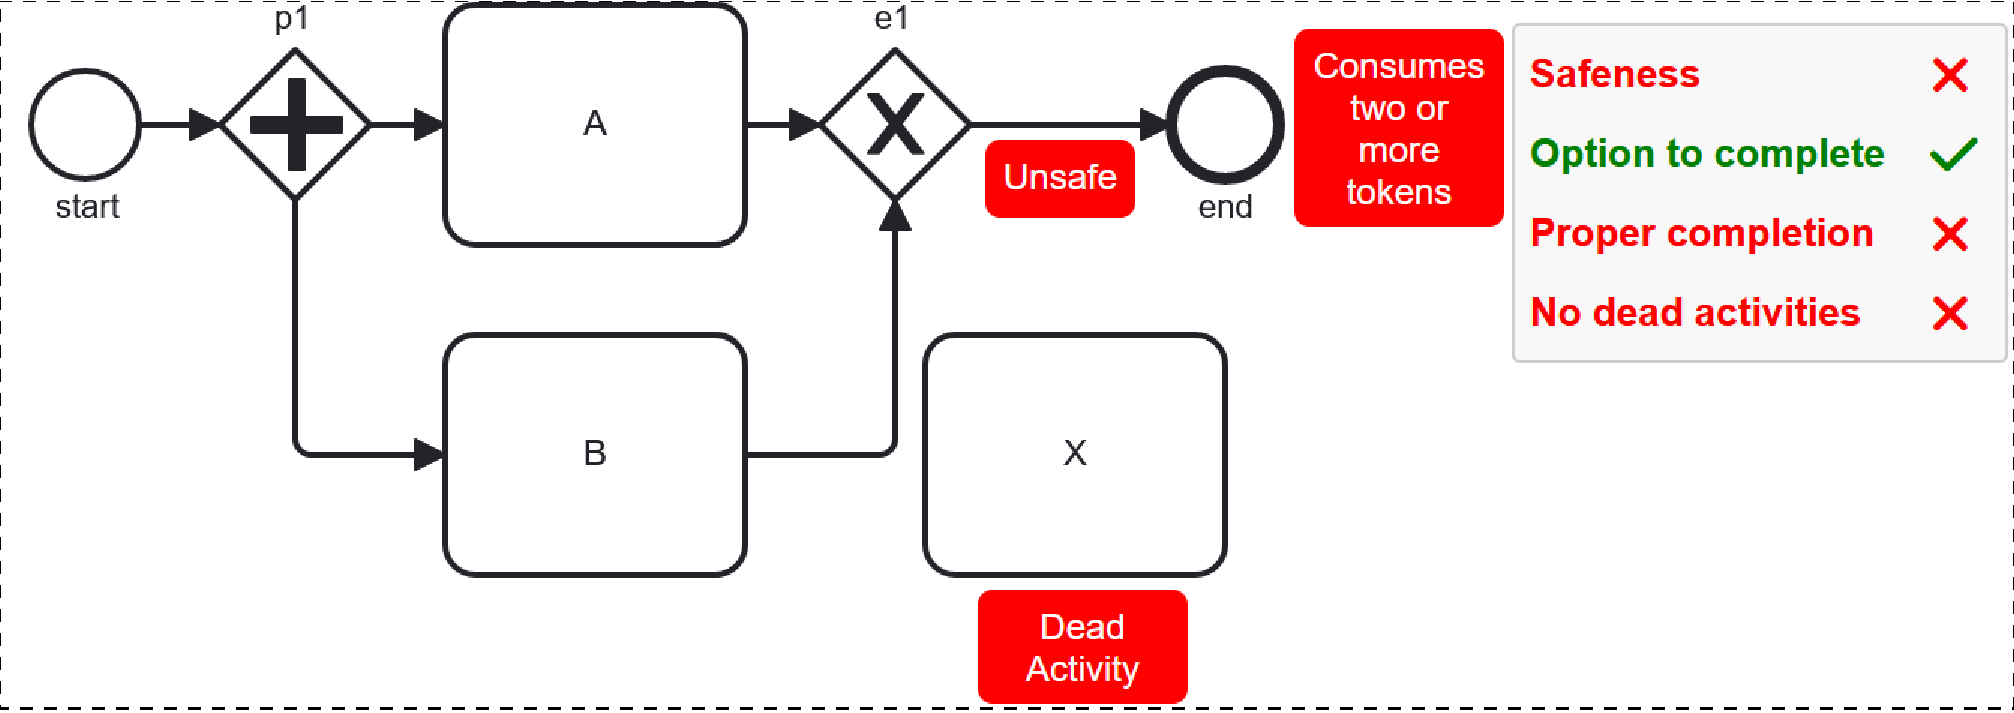
\includegraphics[width=0.9\textwidth]{images/violations}
	\caption{\textit{Soundness violations} in the analysis tool}
	\label{fig:violations}
\end{figure}

Using the overlays, one can immediately see which elements cause soundness violations, which helps to pinpoint the root problems in the BPMN models.
For \textit{safeness}, we highlight sequence flows that can become \textit{unsafe}, i.e., two tokens can be located at the sequence flow.
For \textit{proper completion}, we identify the end events that can consume more than one token.
In contrast, for \textit{no dead activities}, we highlight the dead activities in the BPMN model.
For \textit{option to complete} we cannot highlight elements since it means the process execution can get stuck which cannot easily be attributed to single BPMN elements.
% --> Seen partly in other tools

% Interactive visualization of counterexamples. --> Not seen before. some allow exports of counter-examples but no direct interaction --> friction reduction.
However, just by looking at the BPMN model, it can still be hard to understand soundness violations due to the interplay of the BPMN element's execution semantics.
In the BPMN specification, execution semantics are described using the concept of moving \textit{tokens}~\cite{objectmanagementgroupBusinessProcessModel2013}.
% Universally used token concept
The concept of tokens is used in BPMN tools in the industry to depict process execution information~\cite{camundaservicesgmbhBpmnjsTokenSimulation2024} and in many BPMN formalizations~\cite{corradiniFormalApproachAnalysis2021,houhouFirstOrderLogicVerification2022,krauterFormalizationAnalysisBPMN2023}.

We use tokens in our tool to \textit{interactively} visualize the counter-examples, i.e., violation witnesses of our soundness properties.
Our soundness checker provides counter-examples for all properties besides no dead activities.
Then, we visualize these counter-examples directly in the BPMN editor by showing how tokens move from the process start to a state that violates the given soundness property.
\autoref{fig:counter-example} shows a screenshot visualizing the safeness counter-example for the same BPMN model as shown in \autoref{fig:violations}.

% A bit wasteful regarding space due to the execution log.
\begin{figure}[ht]
	\centering
	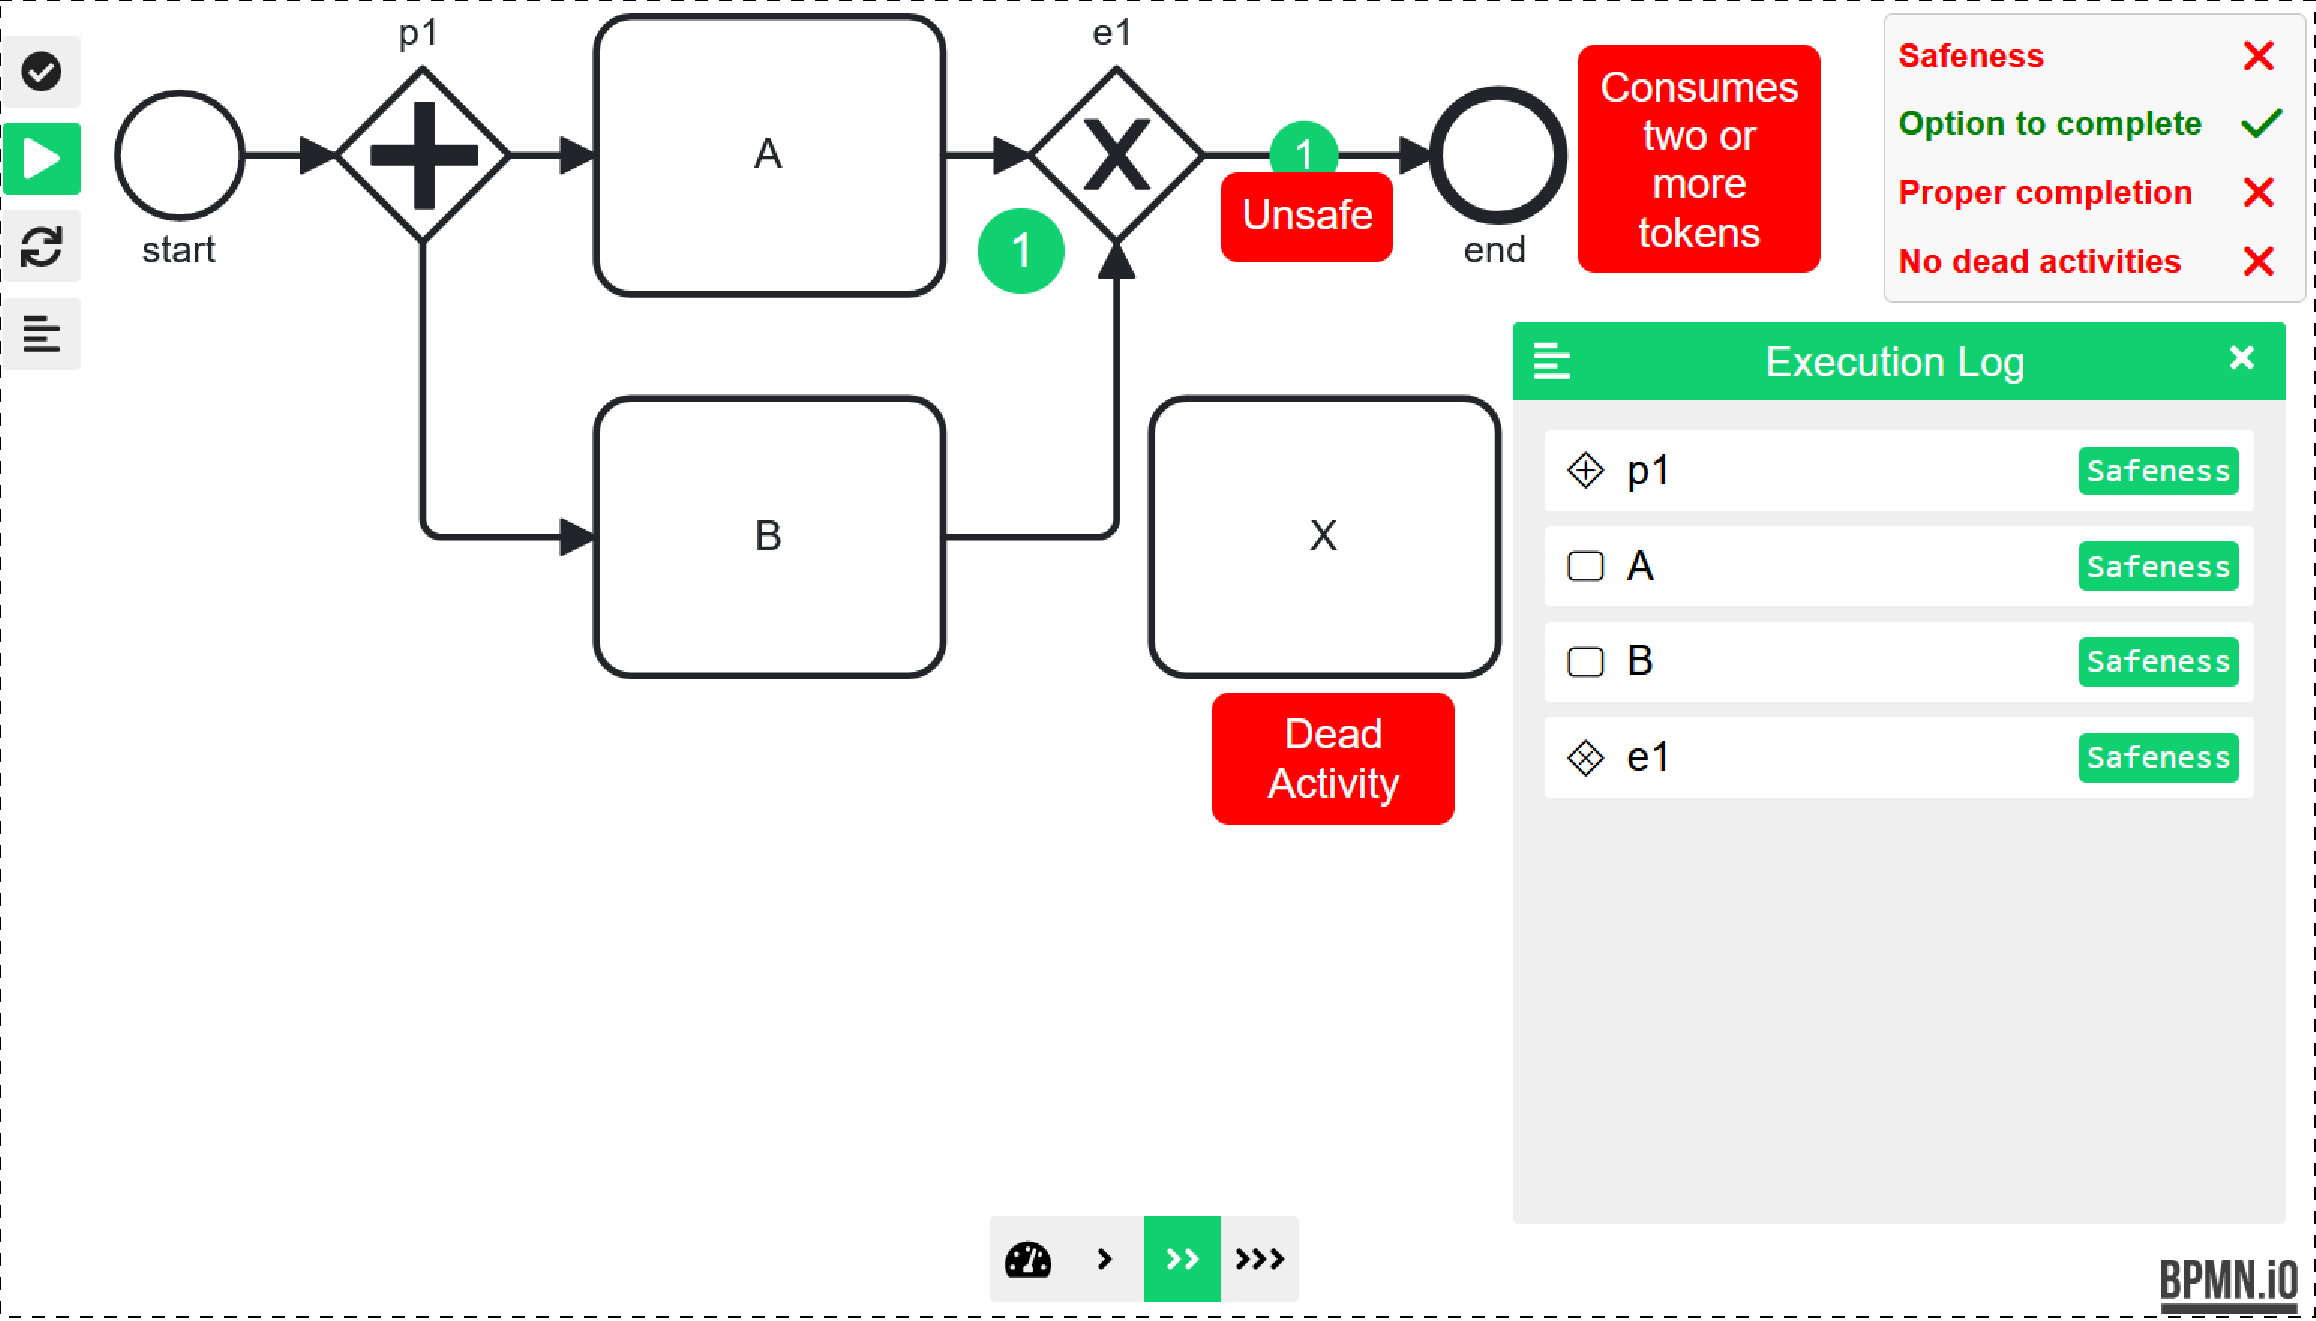
\includegraphics[width=0.9\textwidth]{images/counter-example}
	\caption{Interactive \textit{counter example visualization} in the analysis tool}
	\label{fig:counter-example}
\end{figure}

% Describe the figure.
In \autoref{fig:counter-example}, the visualization has been \textit{paused} just before the \textit{unsafe} state was reached.
One token is already located at the sequence flow, which is marked as unsafe, while a second token is currently waiting at the exclusive gateway \textsf{e1}.
The visualization can be resumed or restarted using the play and restart button on the left side.
When resumed, the gateway \textsf{e1} will execute, resulting in two tokens at the subsequent sequence flow, i.e., an unsafe execution state.
In addition, one can control the visualization speed using the bottom buttons next to the speedometer.

% Execution log
Furthermore, our tool shows an \textit{execution log}, which states the history of BPMN elements being executed.
In \autoref{fig:counter-example} the parallel gateway \textsf{p1}, the activities \textsf{A} and \textsf{B}, as well as the exclusive gateway \textsf{e1} have each been executed once before the pause.
This is useful since often an unsuspected execution order leads to property violations.

% Conclusion for comprehensible
In summary, we aim to make soundness checking quickly \textit{comprehensible} even for users unaccustomed to the BPMN execution semantics.
First, we directly highlight problematic elements in the BPMN editor.
Second, we provide an \textit{interactive} visualization of counter-examples in the BPMN editor with the ability to pause the visualization, control the visualization speed, and show an execution log, which makes understanding the property violation straightforward.

\subsection{Fixable Soundness Checking}

When possible, we detect errors in the BPMN model and provide an automatic fix similar to \textit{quick fixes} in Integrated Development Environments (IDEs).
Modelers can then select these quick fixes to resolve a soundness property violation.
\autoref{fig:quick-fixes} shows a screenshot of our tool, where quick fixes are depicted as green overlays containing a light bulb icon.
This icon is typically used to indicate quick fixes in IDEs.
Our tool simultaneously shows soundness violations (\autoref{fig:violations}) and quick fixes (\autoref{fig:quick-fixes}).

\begin{figure}[ht]
	\centering
	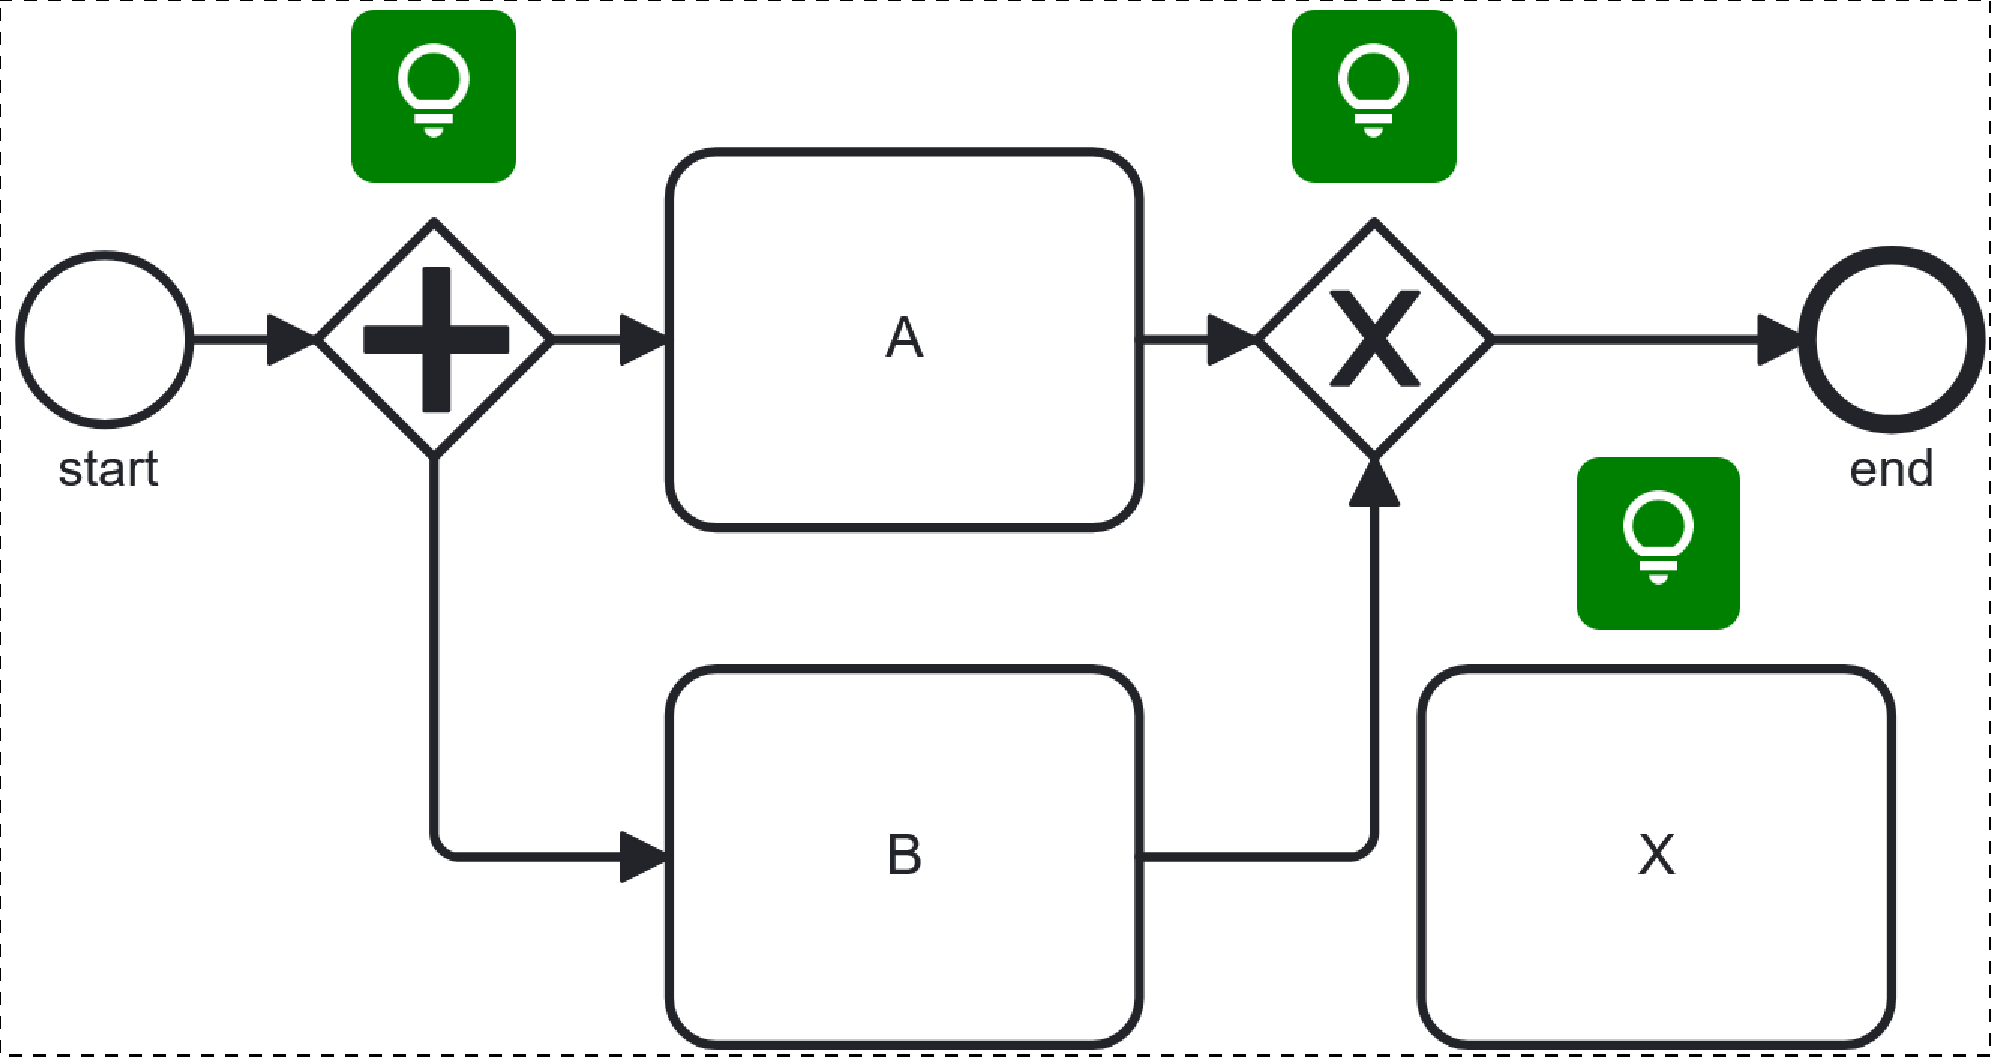
\includegraphics[width=0.6\textwidth]{images/quickfixes}
	\caption{\textit{Quick fixes} in the analysis tool}
	\label{fig:quick-fixes}
\end{figure}

The user can apply a quick fix by clicking on the green overlays and immediately see the changes in soundness since checking is \textit{instantaneous} as discussed in \autoref{subsec:instantaneous}.
If he is unhappy with the result, a user can undo all changes as a whole since each quick fix is a \textit{command}, according to the command pattern.
A user might not like a quick fix if it not only fixes a specific property but also has unintended side effects.
For example, it might invalidate a different soundness property.

In the following sections, we describe the implemented resolution strategies for the different soundness properties in detail.
However, we do not expect these strategies to cover all possible resolutions and fit all applications.
Thus, our framework is extensible, so other developers can provide additional or custom resolution strategies.
This is possible since we \textit{decoupled} the soundness analysis from showing violations and providing quick fixes in our implementation, which facilitates customization by using dependency injection.

\subsubsection{Safeness} \label{subsec:safeness}
The soundness checker will provide a counter-example and identify the unsafe sequence flows.
We use this information together with the structure of the BPMN model to find resolutions for \textit{Safeness} violations.
In general, safeness violations can have multiple reasons.

\begin{enumerate}
	\item An exclusive gateway with multiple incoming sequence flows activated more than once will lead to multiple tokens at its outgoing sequence flows.
	\item One can also implicitly encode an exclusive gateway, for example, using an activity, by having multiple incoming sequence flows.
	Implicitly encoding exclusive gateways is allowed but violates best practices (see lint rule \textit{fake-join} in~\cite{camundaservicesgmbhBpmnlint2024}).
	Similar to \textbf{(1)}, this leads to unsafe sequence flows if activated more than once.
\end{enumerate}


\textbf{Resolutions for (1):} A straightforward solution is to change the exclusive gateway to a parallel one.
Since the gateway was activated multiple times, it indicates that it perhaps should have been a parallel gateway or that there was an unintended parallelization before.
Thus, we can analyze the BPMN model and find the parallelization that causes the \textit{Safeness} violation.
If it is a parallel gateway, another solution is to change this parallel gateway to an exclusive one.
So, there are two solutions, but the goal is to have matching gateways.
The parallelization can also be an implicitly encoded parallel gateway, for example, an activity with multiple outgoing sequence flows, which does not comply with best practices but is allowed.
In this case, we can add an exclusive gateway to eliminate the implicit parallelization and achieve matching gateways.
% It would be nice to mention the command here already.

\textbf{Resolutions for (2):} Similarly to \textbf{(1)}, the goal of each quick fix is to obtain matching gateways.
Thus, one solution is to find the parallelization that causes the \textit{Safeness} violation and change it to an exclusive gateway, as described in \textbf{(1)}.
Quick fix \textbf{(a)} in \autoref{fig:safeness} shows this solution, where a parallel gateway is changed to an exclusive one.
We color all changes and additions green in figures, highlighting quick fixes.
Another solution is to remove the implicit exclusive gateway and add a parallel gateway instead, see quick fix \textbf{(b)} in \autoref{fig:safeness}.
The quick fix moves elements automatically to make space to insert the parallel gateway and then reconnects as well as adds sequence flows accordingly.
Even though these are multiple individual operations, we ensured that an undo operation would revert the entire quick fix.
All the implemented quick fixes can be reverted using one simple undo operation.

\begin{figure}[ht]
	\centering
	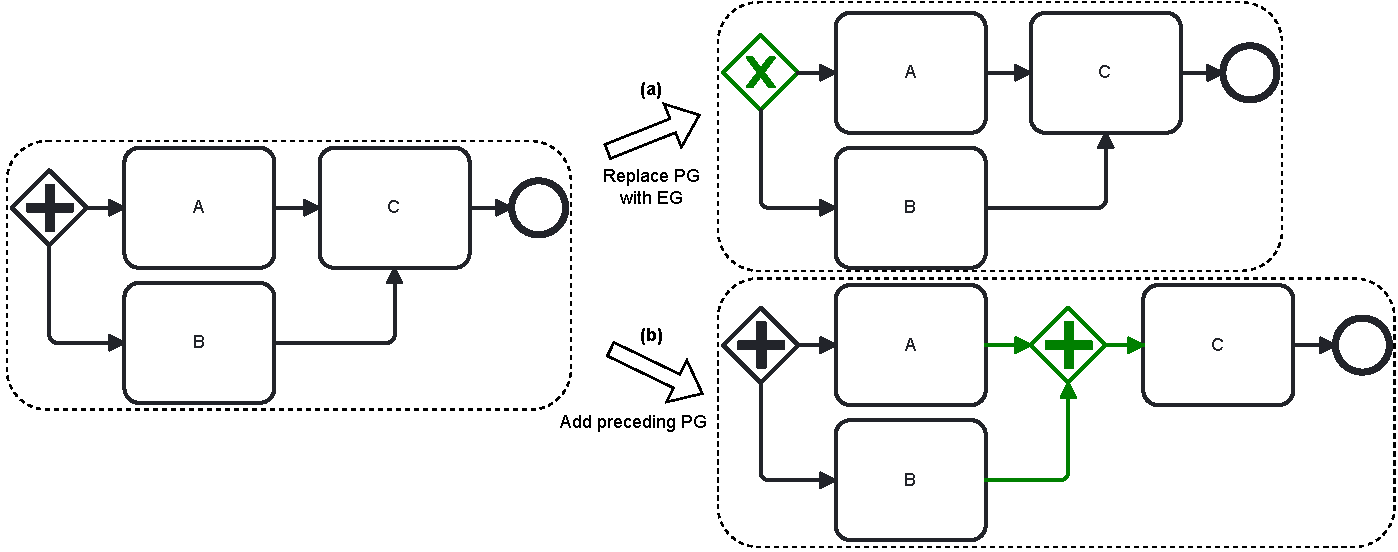
\includegraphics[width=1\textwidth]{images/safeness}
	\caption{Example quick fixes for \textit{Safeness}}
	\label{fig:safeness}
\end{figure}

% TODO: Add demo application and artifacts anonymously.
Our demo application in x contains examples of the Safeness quick fixes and all other soundness properties.

\subsubsection{Proper Completion}
The soundness checker will provide a counter-example and the end events that consume more than one token.
Violations of \textit{Proper Completion} at a specific end event can have multiple reasons.

\begin{enumerate}
	\item An end event can have multiple incoming sequence flows that can hold tokens.
	This could be due to a parallelization that is never synchronized.
	\item If there is only one incoming sequence flow, then this flow must be unsafe, i.e., hold more than one token in a possible execution.
\end{enumerate}

\textbf{Resolution for (1):} If multiple incoming sequence flows are the cause, we can add a unique end event for each except the first.
\autoref{fig:properCompletion} shows an example of this quick fix being applied, where the changed elements are colored in green.
We ensured an undo operation would revert the quick fix using the command pattern.

% Can save a lot of space in this figure if needed. Go to two activities and put them closer together
\begin{figure}[ht]
	\centering
	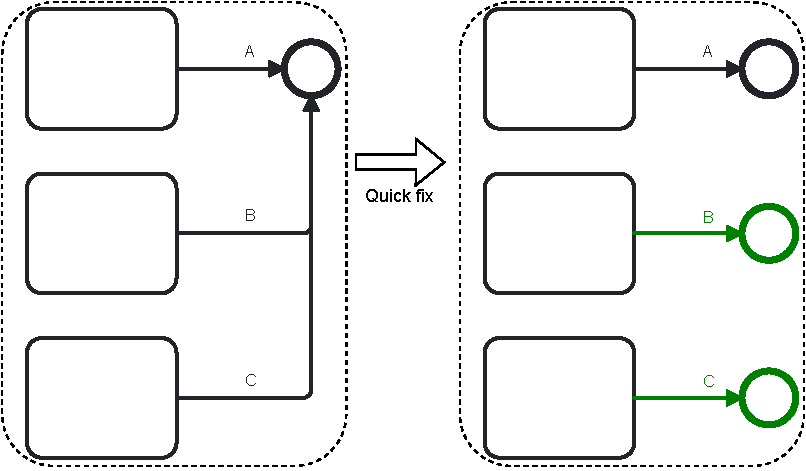
\includegraphics[width=0.7\textwidth]{images/properCompletion}
	\caption{Example quick fix for \textit{Proper Completion}}
	\label{fig:properCompletion}
\end{figure}

\textbf{Resolution for (2):} If a problematic end event only has one incoming sequence flow, it must be unsafe.
Thus, other \textit{Safeness} quick fixes can apply, which will also resolve \textit{Proper Completion}, see \autoref{subsec:safeness}.


\subsubsection{Option to Complete} \label{subsec:optionToComplete}
Violations of \textit{Option to Complete} can have multiple reasons.

\begin{enumerate}
	\item A parallel gateway that synchronizes multiple incoming sequence flows but never executes leads to a violation.
	\item An event that is never triggered but relied upon in the process execution leads to a violation.
\end{enumerate}

To know the reason for a given violation, we analyze the counter example provided by the soundness checker.
The counter-example provides a trace that leads to a state in which the process cannot complete.
By analyzing the last state in this trace, i.e., the state in which execution cannot continue, we can determine which element is the cause.
Thus, we can provide quick fixes for the possible reasons.

\textbf{Resolutions for (1):} A straightforward way to fix sequence flow not continuing past a parallel gateway is to change it from parallel to exclusive.
Exclusive gateways do not synchronize, and thus, execution can continue.
\autoref{fig:optionToComplete} \textbf{(a)} shows an example of this quick fix where the replaced gateway is highlighted in green.

\begin{figure}[ht]
	\centering
	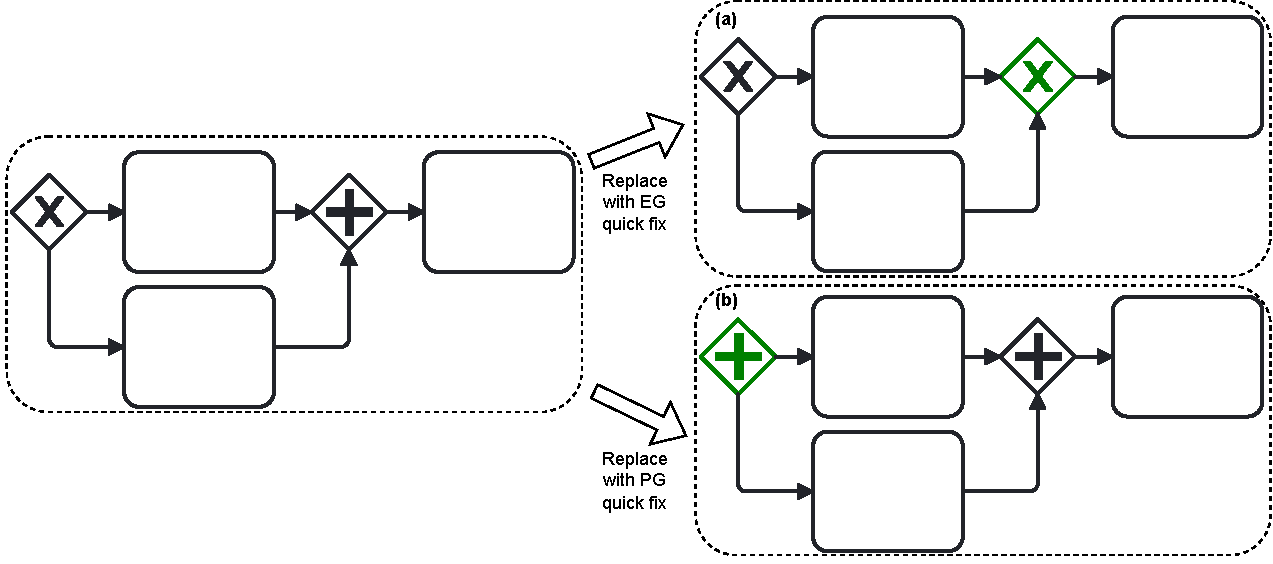
\includegraphics[width=1\textwidth]{images/optionToComplete}
	\caption{Example quick fixes for \textit{Option To Complete}}
	\label{fig:optionToComplete}
\end{figure}

Another way to fix violations is to find the split in the sequence flow, for example, the exclusive gateway in \autoref{fig:optionToComplete}, and make this split a parallelization, see quick fix \textbf{(b)} in \autoref{fig:optionToComplete}.
We present both possible resolutions to the user, who can choose the appropriate one.
Similar to the quick fixes

In the example in \autoref{fig:optionToComplete}, it is possible to spot the mismatching gateways.
However, this might not be straightforward in bigger BPMN models with more flow nodes and sequence flows.

\textbf{Resolutions for (2):} We have not yet implemented any quick fixes for events, but many possibilities exist.
For example, for message catch events without incoming message flows, one could add a fitting message flow from a message throw event or send task.
One can use different factors, such as spatial proximity and name similarity, to find the right source of the new message flow.
The idea for any event would be to add the missing trigger.
Finding the most fitting trigger can be done in various ways by analyzing the other elements in the BPMN model.


\subsubsection{No Dead Activities}
A dead activity might have multiple reasons:

\begin{enumerate}
	\item The simplest reason is that the activity is disconnected, i.e., it has no incoming sequence flow.
	Disconnected activities must not be dead, but they violate best practices see lint rule \textit{no-disconnected} in~\cite{camundaservicesgmbhBpmnlint2024}.
	\item An activity can also be part of the BPMN model that is not reachable during execution because, for example, a parallel gateway preceding the activity cannot be executed.
\end{enumerate}
% Could also be behind events that are never triggered.

\textbf{Resolutions for (1)}: If the activity is disconnected, we can propose connecting it to the nearest flow node.
However, this flow node should not be disconnected or dead itself.

\textbf{Resolutions for (2)}: When the dead activity is connected, this often means it is unreachable during execution, and often the process itself cannot terminate, i.e., violates \textit{Option to Complete}.
Thus, other quick fixes can apply, which will also resolve dead activities, see \autoref{subsec:optionToComplete}.

\section{Implementation}

In this section, we briefly describe and highlight key elements in our implementation of the BPMN soundness checking tool.
The main goal of the tool is to be well integrated into modeling tools without introducing friction in the modeling process.
To achieve this, we keep the design of our tool modular such that one can either fully integrate it, pick only specific features of the tool, or even extend it, for example to add custom quick fix providers.

\subsection{Tool summary}
Our tool is open-source and available as an artifact~\cite{noauthorgivenBPM2024Artifacts2024}.
The tool architecture is shown in \autoref{fig:overview}, while screenshots of our tool with different features enabled are given in \autoref{fig:violations}, \autoref{fig:counter-example}, and \autoref{fig:quick-fixes}.
The front-end of the tool is built in web technologies using the bpmn-js ecosystem~\cite{camundaservicesgmbhBpmnjsTokenSimulation2024}, while the soundness and safeness checking is implemented in the Rust programming language.

We developed the model checking in Rust due to its low memory overhead, absence of garbage collection, and performance comparable to programming languages such as C and C++.
A fast programming language and direct implementation of the BPMN semantics play a key role in achieving \textit{instantaneous} soundness checking of realistic process models.
However, our tool is not yet heavily optimized for performance to avoid code complexity.
In addition, partial-order reduction techniques, common in other model checkers, are not implemented to tackle the state space explosion problem.
% Zero-copy? --> Currently, we are copying things but still achieve better performance (Tradeoff with readability)

Our tool can provide model checking as a \textit{web-service} or command-line application to be integrated with any BPMN modeler.
Otherwise, one can reuse parts of the user interface described in \autoref{sec:soundness}.
This allows many ways to smoothly integrate soundness checking into existing BPMN modeling tools, making it understandable for most BPMN modelers.

\subsection{Pragmatic BPMN Semantics Encoding}
In addition to selecting an efficient programming language for developing the soundness checker, we also opted for a practical, straightforward encoding of BPMN semantics.
Our encoding contains sufficient detail to check soundness and safeness while omitting unnecessary intermediate states, which leads to smaller state spaces.
For example, \autoref{fig:activityEncoding} shows that we do not encode the start and end of a task but rather the execution as a whole.
As discussed earlier, this simple abstraction avoids one additional state and pays off, especially in models with many parallel branches, which can significantly reduce the overall state space.

% This could be made smaller by reducing the space between the flow nodes.
\begin{figure}[ht]
	\centering
	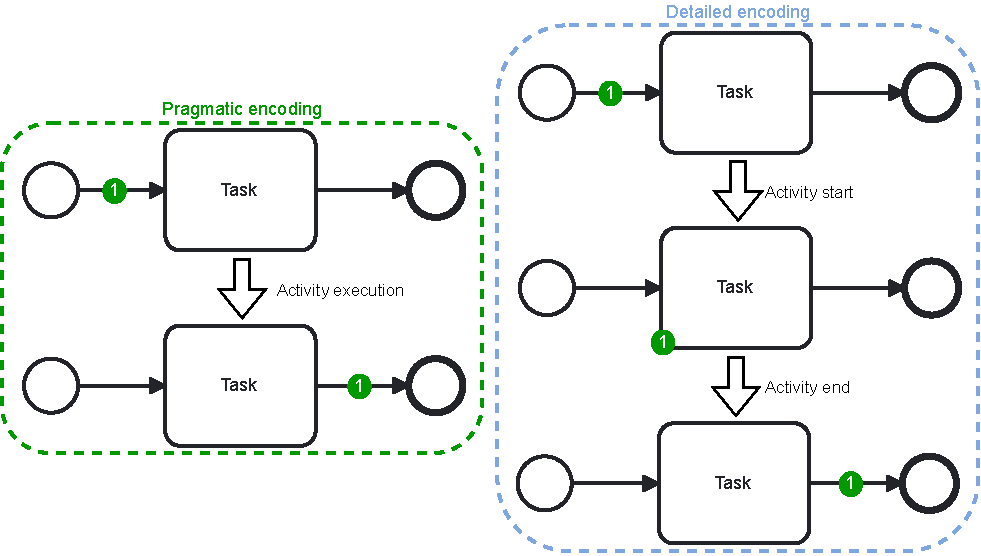
\includegraphics[width=0.7\textwidth]{images/pragmatic-encoding}
	\caption{Pragmatic task execution encoding vs. Detailed encoding}
	\label{fig:activityEncoding}
\end{figure}

% For example: Message start events? Message events in general? Event-based gateways.
We use similar minimal encodings for other BPMN elements related to message flow to keep the state space small.
Nevertheless, one must always be sure that such optimizations do not compromise the checked properties, similar to when applying partial-order reduction techniques~\cite{valmariStateExplosionProblem1998}.

\section{Related Work}

\textbf{BPMN specification coverage:}
Most related work focuses on the BPMN formalization which allows for soundness and safeness checking.
Thus, these approaches show how different BPMN elements can be formalized and compare themselves with each other regarding supported elements~\cite{corradiniFormalApproachAnalysis2021,houhouFirstOrderLogicVerification2022,krauterFormalizationAnalysisBPMN2023,krauterHigherorderTransformationApproach2023}.
The supported BPMN elements come close to the capabilities of popular process orchestration platforms such as Camunda.
Thus, how to formalize nearly all BPMN elements used in practice is straightforward.
Consequently, in this publication, we focus on tool performance and capabilities concerning soundness checking comprehension, resolution, and seamless integration into BPMN modeling tools.

\textbf{Tool performance:}
Comparing tool performance without standardized benchmarks and a reproducible environment is challenging.
However, other publications indicate that tools quickly take several seconds for checking single soundness properties~\cite{corradiniFormalApproachAnalysis2021,houhouFirstOrderLogicVerification2022,krauterHigherorderTransformationApproach2023}.
Our approach checks all soundness properties and safeness of the same models instantaneously.
The difference in performance lies probably in our pragmatic BPMN encoding optimized for soundness checking and the direct implementation in a performant programming language such as Rust rather than a transformation of BPMN to general model checking tools.

\textbf{Tool capabilities:}
Another way to compare the different BPMN formalizations and soundness checking tools is to investigate their capabilities.
Most tools formalize large parts of the BPMN specification and allow soundness and safeness checking~\cite{corradiniFormalApproachAnalysis2021,houhouFirstOrderLogicVerification2022,krauterFormalizationAnalysisBPMN2023,krauterHigherorderTransformationApproach2023}.
Some tools investigate additional aspects such as the introduction of \textit{data} and \textit{time} during verification~\cite{corradiniFormalisingAnimatingMultiple2022,houhouFirstOrderLogicVerification2022}.
Furthermore, other tools allow specifying and checking \textit{custom temporal logic properties}~\cite{corradiniFormalApproachAnalysis2021,krauterFormalizationAnalysisBPMN2023} and even provide graphical interfaces to easy the specification~\cite{krauterHigherorderTransformationApproach2023}
Moreover, some tools provide interactive BPMN simulation using token-flow animation~\cite{camundaservicesgmbhBpmnjsTokenSimulation2024,corradiniFormalisingAnimatingMultiple2022}, while others \textit{visualize counter examples} for soundness violations using tokens~\cite{houhouFirstOrderLogicVerification2022}.

Our tool focuses on \textit{instantaneous} soundness and safeness checking and does not support custom properties or data and time.
We do not provide BPMN simulation since other tools already offer this.
However, we use token-flow animation to visualize counter-examples for soundness violations interactively.
This improves comprehension compared to previous static, less interactive visualizations.
In addition, to the best of our knowledge, our tool is the only one that provides \textit{quick fixes}, i.e., automatic resolutions if soundness properties are violated.
To sum up, our tool incorporates several ideas from the state of the art while enhancing them with novel concepts.
However, the most crucial aspect of our tool is its practical approach that prioritizes performance and understanding above all else to ensure seamless integration into BPMN modeling tools.

\section{Limitations \& Threats to Validity}
% Limitations
Assessing tool performance becomes difficult when there are no standardized benchmarks for comparison.
In this publication, a direct comparison of our tool's performance with related work is not feasible.
This is due to variations in benchmark conditions, such as hardware, operating systems, and employed methodologies.
Thus, we claim that our tool can deal with most BPMN models instantaneously, as previously discussed.
It is advisable to consider the results reported by other researchers on the same models only as a general reference.
To solve this problem we advocate for defining a standardized benchmarking process to directly and transparently compare tool performance.

% External validity instantaneous soundness checking: 
The main threat to the external validity~\cite{wohlinExperimentationSoftwareEngineering2012} of our instantaneous soundness checking claim is that we could not test our tool with a large set of models from an industrial setting.
To mitigate this threat, we validated our claim against models sourced from existing literature, public repositories, and two artificial datasets featuring extensive and complex BPMN models.
We believe these datasets closely resemble or even surpass industrial models in terms of model size and complexity (state space).

Furthermore, regarding comprehensive soundness checking, we plan to study how well modelers understand soundness violations using the provided highlighting and interactive visualization and how the provided quick fixes impact the resolution.

\section{Conclusion \& Future work}

% Benchmarks in the instantaneous section are a contribution --> We even provides tools to generate more models.

% Future work: Ranking quick fixes (least change, learn from the user, etc.)
% Future work: Quick fixes for more complex BPMN features. We only looked at gateways/end events being problematic so far.
% Problems: Only checking four properties, not custom properties
% Loops for quick fixes?

\bibliographystyle{splncs04}
\bibliography{bib}

\end{document}
